\graphicspath{{./lab05/Images/}}


\maketitlepage{App Development}{in Android Studio}{Lab 5: Storage}
\maketocpage

\section{Shared preferences}
If the data we need to store is small and fits into key-value pairs then \texttt{SharedPreferences} is ideal. It is a very simple way to read and write data. A \texttt{SharedPreference} instance references a file on the phone which includes key-value pairs. These preferences can be bound to a single app or shared between many. From an activity, we can access preferences in the following way.
\begin{lstlisting}[style=A_Java]
// Shared preferences
SharedPreferences pref1 = getSharedPreferences("MY_PREF", MODE_PRIVATE);
// Preferences
SharedPreferences pref2 = getPreferences(MODE_PRIVATE);
\end{lstlisting}
The first can be shared between multiple activities and has its own identifier while the latter is an activity's default preference. The \texttt{MODE\_PRIVATE} flag determines the accessibility to the preference, which in this case is only the current app. Others include \texttt{MODE\_WORLD\_READABLE} and \texttt{MODE\_WORLD\_WRITEABLE} which allow other apps to read and write to the preference respectively. To access the data in a preference, we can use various methods depending on the value type.
\begin{lstlisting}[style=A_Java]
SharedPreferences pref = getSharedPreferences("MY_PREF", MODE_PRIVATE);
// -1 is the default value if key is not found
int val1 = pref.getInt("some_key_1", -1);
boolean val2 = pref.getBoolean("some_key_2", false);
Map<String, ?> allPairs = pref.getAll();
\end{lstlisting}
To write to a preference we must use a preference editor.
\begin{lstlisting}[style=A_Java]
SharedPreferences pref = getSharedPreferences("MY_PREF", MODE_PRIVATE);
SharedPreferences.Editor editor = pref.edit();
editor.putString("MY_KEY", "MY_VALUE");
editor.apply(); // happens in background, use .commit() to force write here
\end{lstlisting}
In the provided example we use \texttt{SharedReferences} to store background color settings so when the app is started again the color is set to whatever it was the last time the app was used. The sourcecode is available \href{https://github.com/JonSteinn/AndroidDevelopment/tree/master/examples/lab5/colorpref}{here} and a programming session \href{TODO}{here}.

\section{Local SQLite database}
Android has a built in local SQLite database. SQLite is an very small and lightweight ACID-compliant open source relational database system written in C. This course assumes prior knowledge of databases and SQL. The main objective here is to use them in Android so most table schemas are kept trivial.\\

Since the database is local, it can not be used to share resources between various users of an app. It can still be useful to store data locally and an offline app would be a prime example. It is faster than a remote database but should still be performed asynchronously. We will look at two approaches to using the local database. 

\subsection{SQLite APIs}
The SQLite APIs are somewhat low level and often use raw SQL queries. We will use SQLiteOpenHelper, which require an App Context, to create a database and its tables and add to it some access methods.

\begin{lstlisting}[style=A_Java]
public class DbHelper extends SQLiteOpenHelper {
    public DbHelper(Context context) {
        super(context, "MY_DATABASE.db", null, 1);
    }
    @Override
    public void onCreate(SQLiteDatabase db) {
        db.execSQL("CREATE TABLE PERSONS (ID INTEGER " +
                "PRIMARY KEY AUTOINCREMENT, NAME TEXT)");
    }
    @Override
    public void onUpgrade(SQLiteDatabase db, int oldV, int newV) {
        db.execSQL("DROP TABLE IF EXISTS PERSONS");
        onCreate(db);
    }
    public void deletePersonById(String id) {
        SQLiteDatabase db = getWritableDatabase();
        db.delete("MY_DATABASE.db", "ID = ?", new String[]{id});
        db.close();
    }
    public List<String> getAllUsers() {
        SQLiteDatabase db = getReadableDatabase();
        Cursor c = db.rawQuery("SELECT NAME FROM PERSONS", null);
        List<String> lis = new ArrayList<>(c.getCount());
        while (c.moveToNext()) lis.add(c.getString(1)); // 0 = ID, 1 = NAME
        c.close();
        db.close();
        return lis;
    }
}
\end{lstlisting}
Note that getting a new \texttt{SQLiteDatabase} instance in each access method is expansive so you might want to use a single instance and close it when done. In the provided example we create a single table database holding game info which you can add to, edit and remove. The source code is available \href{https://github.com/JonSteinn/AndroidDevelopment/tree/master/examples/lab5/gamesdb}{here} and a programming session \href{TODO}{here}.

\subsection{Room Persistence Library}
The Room persistence library provides an abstraction layer over SQLite. It was introduced by Google in 2017\footnote{There could be some Java +1.8 compatability issues depending on when you are reading this}. It uses annotation and consists of the three following components.

\begin{itemize}
\item \textbf{Database}. Contains the database holder and serves as the main access point for the underlying connection to your app's data.
\item \textbf{Entity}. Represents a table within the database.
\item \textbf{DAO}. Contains the methods used for accessing the database.
\end{itemize}

\begin{figure}[H]
\centering
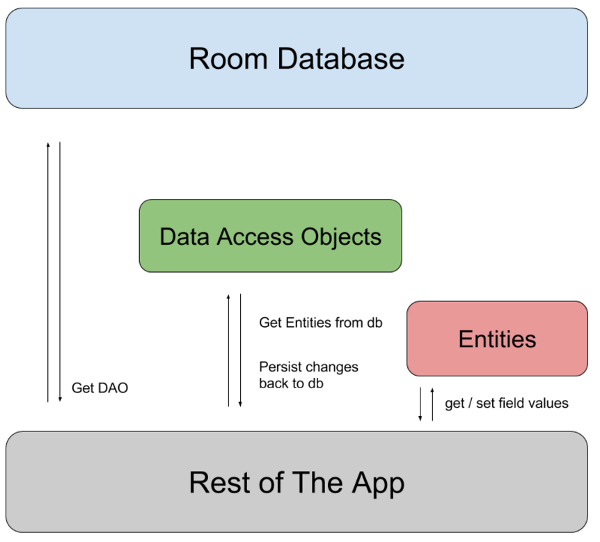
\includegraphics[scale=0.4]{room_architecture.png}
\caption{Room's architecture}
\label{fig:roomarch}
\end{figure}

Add the following dependencies to your \texttt{build.gradle} but make sure to use the latest versions.
\begin{lstlisting}[style=A_txt]
compile 'android.arch.lifecycle:extensions:1.0.0'
compile 'android.arch.persistence.room:runtime:1.0.0'
annotationProcessor 'android.arch.lifecycle:compiler:1.0.0'
annotationProcessor 'android.arch.persistence.room:compiler:1.0.0'
\end{lstlisting}
The following shows a very simple \texttt{Entity} where the table has only two columns, an auto generated id and a name.
\begin{lstlisting}[style=A_Java]
@Entity(tableName = "PERSONS")
public class Person {
    @PrimaryKey(autoGenerate = true)
    private int id;

    private String name;

    // + getters&setters and possibly a constructor
}
\end{lstlisting}
The access object contains various methods to access our data. In the following example we have a way to get all, get a specific person, delete one and add one.
\begin{lstlisting}[style=A_Java]
@Dao
public interface PersonDAO {
    @Query("SELECT * FROM PERSONS")
    List<Person> getAll();

    @Query("SELECT * FROM PERSONS WHERE name = :name")
    List<Person> getPersonsByName(String name);

    @Delete
    void delete(Person person);

    @Insert(onConflict = OnConflictStrategy.REPLACE)
    void addUser(User user);
}
\end{lstlisting}
Finally we have the database object. Note that in this case we allow queries on the main thread just for testing the database but this should never be allowed in general.
\begin{lstlisting}[style=A_Java]
@Database(entities = {Person.class}, version = 1)
public abstract class MyDatabase extends RoomDatabase {
    public abstract PersonDAO personDao();

    public static MyDatabase getInstance(Context context) {
        return Room.databaseBuilder(context, MyDatabase.class, "MY_ROOM_DB")
                .allowMainThreadQueries() // DON'T ALLOW THIS!
                .build();
    }
}
\end{lstlisting}
In the provided example we create a trivial authentication system (passwords stored as plain text) with Room. We will also allow main thread queries for simplification. The source code is available \href{https://github.com/JonSteinn/AndroidDevelopment/tree/master/examples/lab5/roomdb}{here} and a programming session \href{TODO}{here}.

\section{Remote Firebase databse}
Firebase is a web and mobile development platform owned by Google. It has multiple services like authentication and a realtime database. We will look at the latter, a backend as a service, similar to Azure.\\

The realtime database is a NoSQL database that uses JSON structure to store data. The data is synchronized in realtime to every connected client. To setup Firebase realtime database in your project, go to \menu{Tools > Firebase} and follow the provided instructions. The provided example uses just a single key in the JSON object and sets up a onDataChange listener to it and offers the user to redefine its value. The source code can be found \href{https://github.com/JonSteinn/AndroidDevelopment/tree/master/examples/lab5/firebase}{here} and a programming session \href{TODO}{here}.

\section{Assignment}
In this assignment you can choose between using the local SQLite database or the Firebase realtime database. Your app should start with a simple authentication where a user can create an account or log in with an existing one (a password is not required but usernames must be unique). After that, you get a random arithmetic problem from the following categories:
\begin{itemize}
\item addition
\item subtraction
\item multiplication
\item division
\end{itemize}
The user should be able to enter an answer and you should keep statistics for each category (total wins and total played in category $X$). If a player leaves without answering a question, that question should remain when he comes back. You should also offer the user to view his statistics.